\documentclass[12pt]{article}
\usepackage{graphicx}
\graphicspath{.}

\begin{document}

\section*{Modelo Conceptual}

\subsection*{¿Para qué sirve?}
Los modelos conceptuales son la etapa transitoria entre el modelo orientado hacia el
usuario o cliente y el modelo físico de la Base de Daots. A diferencia del modelo 
Relacional este modelo tiene algunos elementos clave que harán la implementación de 
esta mucho más fácil para el administrador de la Base de Datos.

\subsection*{¿De qué se compone?}
El modelo se caracteriza por agregar los siguientes elementos por sobre el modelo
Relacional que vimos previamente:
\\\\
1) Definición de Atributos y Tipos.
\\\\
2) Claves de tipo Primaria, Foránea y Múltiple.
\\\\
3) Normalización y Desnormalización.
\\\\
Además, este modelo se caracteriza por remplazar los rectángulos y elipses de el 
modelo Relacional por tablas, acercándose más a lo que sería la implementación en 
código, ya sea por SQL u otro sistema.

\newpage

\section*{Notacion UML}
UML es un acrónimo de "Unified Modeling Language", creado con la intención de 
modelar un sistema de relaciones y clases, se usa generalmente para Bases de Datos 
y también para modelar sistemas orientados a objetos. Para poder convertir un 
esquema de tipo relacional a uno de tipo conceptual (en formato UML), debemos usar 
los siguientes pasos:
\\\\
1) Convertir cada Entidad en una tabla.
\\\\
2) Las Entidades Asociativas se convertirán en una nueva Entidad, la cuál se 
colocará entre las otras dos.
\\\\
3) Las Herencias se convertirán en flechas, las cuáles apuntarán a la Super-Clase. 
Si es de tipo Herencia Completa, la Super-Clase se etiqueta como abstracta.
\\\\
4) Las Relaciones se representarán por una linea, en donde la cardinalidad se 
representará con um número en cada extremo de ésta.
\\\\
5) Las Agregaciones se representarán con una relación, la cuál invoca en un rombo 
(sin relleno) que apunta la Entidad Débil.
\\\\
6) Las Composiciones se representarán de la mísma manera que en el punto anterior 
(pero con un rombo relleno).
\\\\

\newpage

\section*{Atributos Clave}
En esta sección se cubren los atributos de cada entidad que darán paso al modelo 
Lógico y finalmente a la implementación física de nuestra Base de Datos.

\subsection*{Dependencia Funcional}
Una dependencia funcional ocurre cuando tenemos una tupla o lista de elementos,
dentro de los cuáles una sublista de ésta se puede representar en función de otra
sublista contenida en la mísma tupla inicial.
\begin{center}
Ejemplo: Persona(RUT, nombre, apellido, dirección).
\end{center}
Podemos notar que si definimos los atributos de esta Entidad Persona, existirá una
dependencia funcional de la siguiente forma: 
\begin{center}
	$RUT \Rightarrow nombre, apellido$ 
\end{center}

\subsection*{Dependencia Parcial}
Una dependencia parcial ocurrirá dentro de una dependencia funcional cuando hayan 
atributos dentro de la clave que formen una dependencia entre otros atributos 
no-clave por si solos.
\begin{center}
Ejemplo: Inventario(ID\_producto, ID\_bodega, descripción, cantidad).
\end{center}
Aquí podemos notar que el atributo ID\_producto forma una dependencia funcional con
descripción, ya que no es necesario tener el ID\_bodega.
\begin{center}
	$ID\_producto \Rightarrow descripción$ 
\end{center}

\subsection*{Dependencia Transitiva}
Una dependencia transitiva ocurrirá cuando exista una dependencia funcional entre un
atributo no-clave y otro atributo no-clave.
\begin{center}
Ejemplo: Empleados(RUT, nombre, ID\_depto, nombre\_depto).
\end{center}
Aquí podemos notar que el atributo ID\_depto forma una dependencia funcional con
nombre\_depto, ambos siendo atributos no-clave.
\begin{center}
	$ID\_depto \Rightarrow nombre\_depto$ 
\end{center}

\subsection*{Grupos Repetitivos}
Los grupos repetitivos ocurrirán cuando haya información redundante dentro de las tuplas
u atributos de una relación, provocando que la búsqueda, modificacíon o eliminación de
datos se haga más compleja e ineficiente.

\begin{center}
Ejemplo: Alumnos(ID, apellido, carrera, codigo\_carrera).
\end{center}
Aquí ocurrirá el fenómeno dentro de los atributos carrera y código\_carrera, ya que estos
datos no solo se repetirán varias veces por cada alumno que haya, si no que también son
datos que probablemente existan dentro de una o más tablas, provocando redundancia y los
problemas previamente mencionados.

\begin{center}
	Alumnos(ID, apellido, \{carrera, codigo\_carrera\}).
	\\
	Carreras(codigo\_carrera, carrera, matriculados).
\end{center}

\newpage

\subsection*{Clave Primaria}
Dicho esto, podemos definir como Clave a un Atributo de cierta Entidad si se cumplen
las siguientes condiciones:
\\\\
1) Existe una dependencia funcional desde esta tupla hacia todos los otros atributos
de la Entidad.
\\\\
2) No existe ninguna sublista de esta tupla que cumpla con la condición anterior
(se dice minimal si es que esto se cumple).
\\\\
Luego, se dice que la clave es Simple si es que se compone de un único atributo y
Compuesta si está compuesta de una tupla de atributos. La clave que identifica una Entidad
se denomina Clave Primaria. Finalmente, si una clave no es minimal, se le llama 
Super-Clave.
\\\\
Una clave primaria también indica como se almacenará el dato en disco, esencialmente
los datos se almacenan de la mísma forma que en una tabla de Hashing; ordenándose por el
valor de su Clave Primaria.

\subsection*{Clave Foránea}
Una clave foránea es, en práctia, una referencia o puntero hacia un Dato o Entidad del mísmo
o diferente tipo. Ésto se logra utilizando la Clave Primaria del otro objeto, y definiéndolo
como un atributo de la clave que la referencia.
\\\\
Sin embargo, por muy útil que sea este concepto, tiene ciertas debilidades; primero, puede
crear una restricción existencial, oséa que si el objeto al cuál se referencia se elimina, 
pueden haber problemas entre las entidades. Y segundo, puede crear un efecto en cascada al 
hacer un UPDATE o DELETE.

\newpage

\section*{Modelo Lógico}
El modelo Lógico se encuentra una vez se hayan realizado las transformaciones necesarias al
modelo Conceptual. Dichos pasos son:
\\\\
1) Toda Relación se transforma una Entidad con Clave Primaria.
\\\\
2) Toda Relación Fuerte-Débil se transforma una asociación de tipo Clave Primaria - Foránea.
\\\\
3) Las Relaciones 1:1 comparten Clave para identificación.
\\\\
4) Las Relaciones 1:N comparten Clave Primaria - Foránea.
\\\\
5) Las Relaciones M:N crean una Entidad nueva que contiene Claves Foráneas hacia las dos 
Entidades.
\\\\
6) Las Relaciones N-arias hacen lo mismo que el punto anterior.
\\\\
7) Las Herencias se cambian a Relaciones 1:1.
\\\\
8) Las Composciciones y Agregaciones se cambian a Relaciones 1:N.
\\\\
9) Las Entidades Asociativas se transforman en Relaciones.

\newpage

\section*{Normalización}
La normalización es un proceso iterativo de remoción de anomalías en el modelo relacional,
el cuál produce un modelo con más relaciones, que a su vez tienen menos atributos. La etapa
de normalización sigue los siguientes pasos:

\begin{center}
	Tabla con valores multi-valuados \\\\
	$\bigg\downarrow$ \\\\
	Primera Forma Normal \\\\
	$\bigg\downarrow$  \\\\ 
	Segunda Forma Normal \\\\
	$\bigg\downarrow$  \\\\
	Tercera Forma Normal \\\\
	$\bigg\downarrow$  \\\\
	Forma Normal Boyce-Codd \\\\
	$\bigg\downarrow$  \\\\
	Cuarta Forma Normal \\\\
	$\bigg\downarrow$  \\\\
	Quinta Forma Normal
\end{center}
\\\\
Es importante recalcar que el modelo no necesariamente parte desde el primer paso, el modelo
puede empezar en cualquiera de los pasos anteriormente mencionados.

\newpage

\subsection{Cero Forma Normal}
Esta forma normal se caracteriza por tener atributos que son multi-valuados, es decir, un
grupo repetitivo dentro de una mísma relación. Para pasar este caso a la primera forma, se 
crea una nueva entidad que contenga el grupo repetitivo y la clave de la entidad original.

\subsection{Primera Forma Normal}
En esta forma normal todos los atributos de la relacion son uni-valuados. Esta forma normal
tendrá dependencias parciales y para pasarlo a la segunda forma normal será necesario crear
una nueva entidad para cada una de estas.

\begin{center}
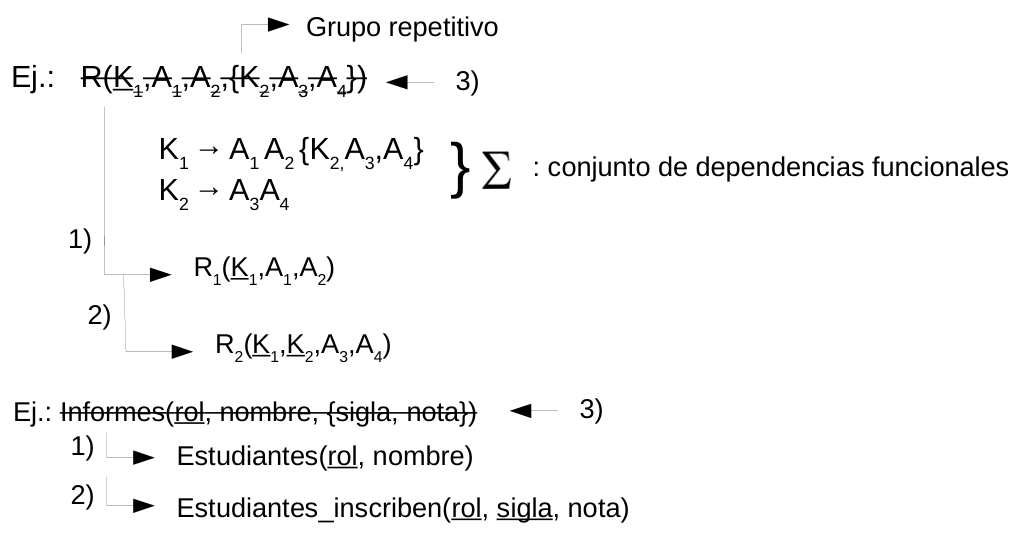
\includegraphics[scale=0.25]{1FN.png}
\end{center}

\subsection{Segunda Forma Normal}
Para este paso, todas las relaciones se definen por tener una clave simple, oséa que la
entidad completa se puede identificar a partir de un único atributo. Esta forma tendrá
dependencias transitivas y para pasarlo a la tercera forma será necesario quedarse con
la clave de la dependencia transitiva como una clave foránea y crear una nueva entidad
que contenga todos los atributos que conformaban dicha dependencia.

\begin{center}
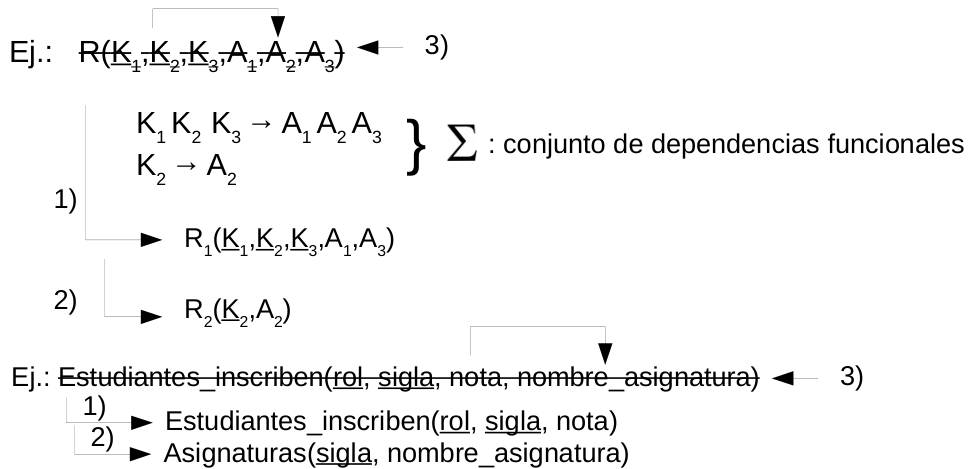
\includegraphics[scale=0.25]{2FN.png}
\end{center}

\subsection{Tercera Forma Normal}
Una relacion se encontrará en esta forma si es que no hay dependencias transitivas
entre elementos no-clave y elementos clave. Para pasarlo a la forma normal Boyce-Codd 
será necesario realizar una rotación, lo cuál implica intercambiar el elemento
no-clave por el clave.

\begin{center}
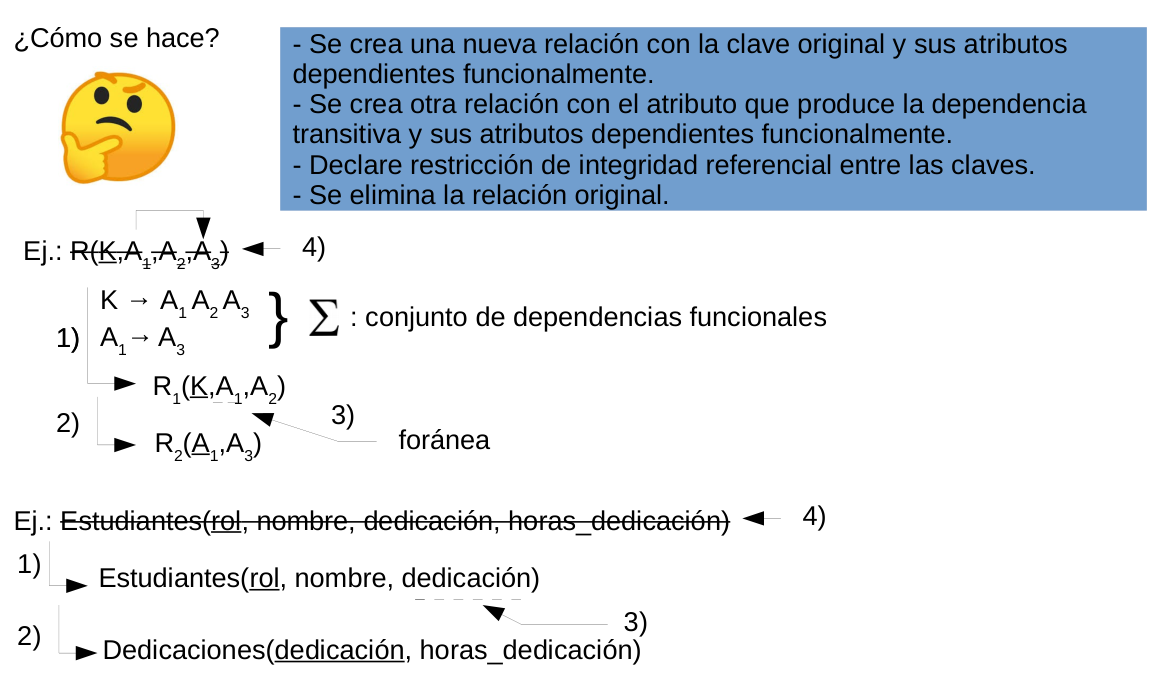
\includegraphics[scale=0.25]{3FN.png}
\end{center}

\subsection{Forma Boyce-Codd}
Aquí las claves permitirán conocer cualquier relación en el modelo con tan solo saber
las claves candidatas, ya que éstas son los únicos descriptores de la relación. Para 
pasar a la cuarta forma normal habrá que transformar todas las dependencias multivaluadas en 
dependencias funcionales. Esto último se logrará invtirtiendo las dependencias mutli-valuadas,
removerlas de la función original y finalmente definir la integridad referencial 
primaria-foránea.

\subsection{Cuarta Forma Normal}
Se dice que un modelo está en cuarta forma normal si es que toda dependencia multivaluada
es una dependencia funcional, es decir, por cada dependencia individual entre dos atributos,
éstas últimas se convierten en una nueva entidad con las claves invertidas. Para convertir
esta forma a la quinta y última forma normal habrá que descomponer las dependencias
conjuntas de la relación, dejándolas en función a la o las claves candidatas.

\subsection{Quinta Forma Normal}
Finalmente, la quinta forma normal denota que el modelo está completamente normalizado y por
ende ya no habrán más pasos por realizar.
\begin{center}
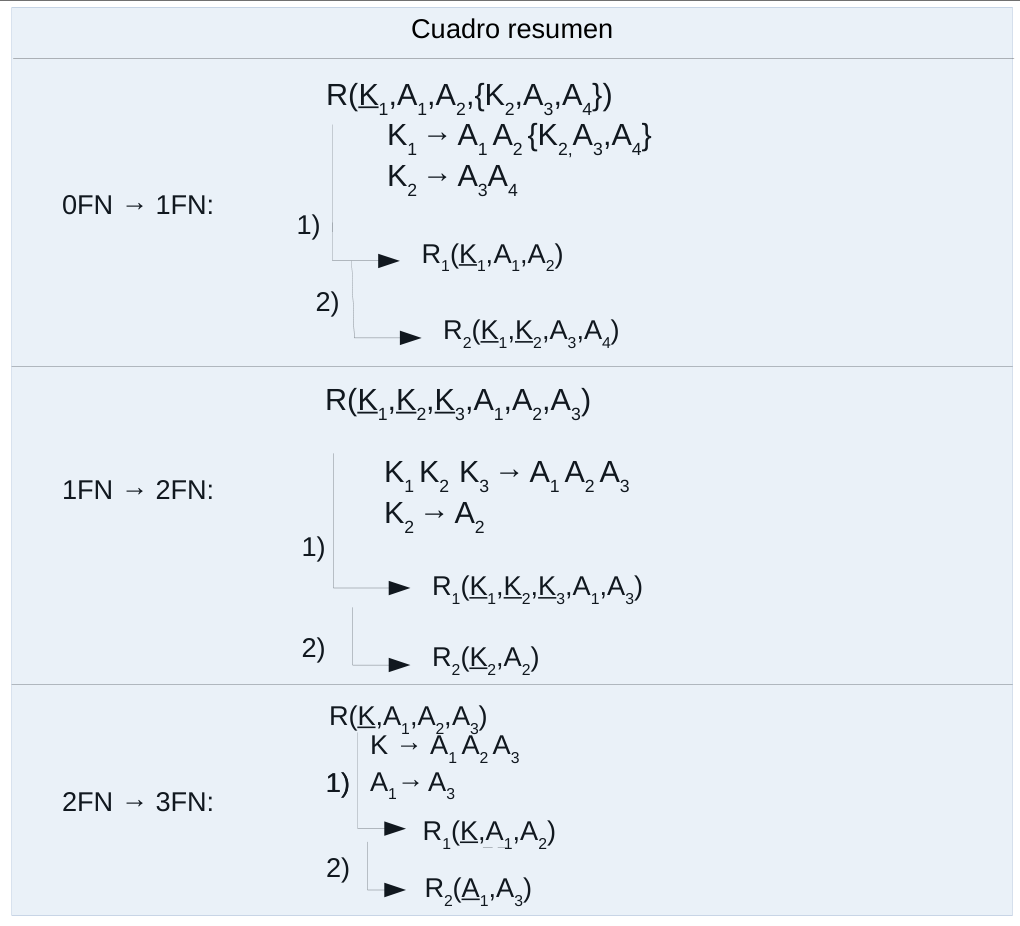
\includegraphics[scale=0.25]{cuadro_resumen.png}
\end{center}

\newpage

\section*{Conceptos Importantes}
Antes de seguir con la siguiente fase de modelamiento es importante denotar los siguientes
conceptos:

\subsection*{Anidamiento}
Corresponde a la búsqueda de datos en una relación a partír de uno o más parámetros. Dependiendo
de la forma en la que se aniden o se calzen los conjuntos de tablas podemos encontrar los siguientes
anidamientos, denominados "Join":

\begin{center}
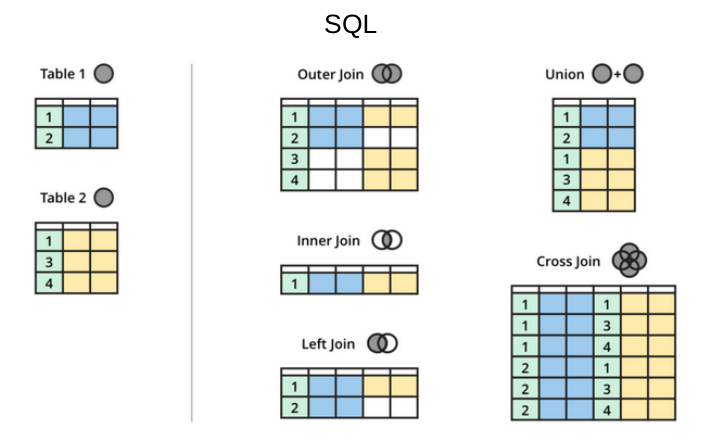
\includegraphics[scale=0.25]{join.png}
\end{center}

\subsection*{Metodología C.R.U.D.}
Patrón de precedencia en SQL, las siglas corresponden a "CREATE", "READ", "UPDATE" y "DELETE".

\subsection*{Ejecución de Consultas}

\begin{center}
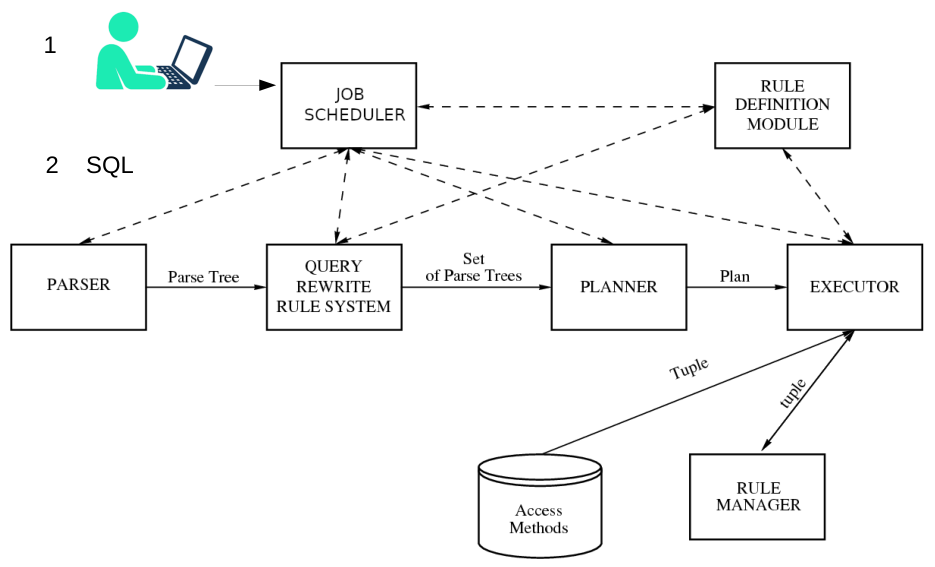
\includegraphics[scale=0.25]{consultas.png}
\end{center}

\newpage

\section*{Modelado Bottom-Up}
Estrategia de procesamiento de información que parte desde la información más detallada y construye
hacia arriba con información cada vez más grande y compleja. En particular se sigue la idea a
continuación:
\\\\
- Extraer los atributos de las vistas físicas e identificar las relaciones.
\\
- Determinar las dependencias funcionales.
\\
- Normalizar el modelo.
\\
- Determinar las asociaciones y su cardinalidad.

\end{document}

